\documentclass[10pt,a4paper]{article}
\usepackage[T1]{fontenc}
\usepackage{lmodern}
\usepackage[margin=1.7cm]{geometry}
\usepackage{amsmath,amssymb}
\usepackage{booktabs,array,tabularx}
\usepackage{enumitem}
\usepackage[dvipsnames]{xcolor}
\usepackage{tikz}
\usetikzlibrary{arrows.meta,positioning,shapes.geometric,calc}
\usepackage[most]{tcolorbox}
\usepackage{fancyhdr}
\usepackage[colorlinks=true,linkcolor=NavyBlue,urlcolor=NavyBlue]{hyperref}

\setlist{nosep,leftmargin=*}
\setlength{\parindent}{0pt}
\setlength{\parskip}{3pt}
\setlength{\emergencystretch}{3em}

\pagestyle{fancy}
\fancyhf{}
\lhead{\small BACSE202 -- Module 3}
\rhead{\small Query Optimization}
\cfoot{\thepage}

\newtcolorbox{keybox}[1][]{colback=NavyBlue!5,breakable,colframe=NavyBlue!70,fonttitle=\bfseries,title={#1},boxsep=2pt,left=4pt,right=4pt,top=2pt,bottom=2pt}
\newtcolorbox{exbox}[1][]{colback=ForestGreen!5,breakable,colframe=ForestGreen!70,fonttitle=\bfseries,title={#1},boxsep=2pt,left=4pt,right=4pt,top=2pt,bottom=2pt}
\newtcolorbox{warnbox}[1][]{colback=BrickRed!5,breakable,colframe=BrickRed!70,fonttitle=\bfseries,title={#1},boxsep=2pt,left=4pt,right=4pt,top=2pt,bottom=2pt}

\newcommand{\R}[1]{\mathrm{#1}}
\newcommand{\aq}{\text{'Aquarius'}}
\newcommand{\bd}{\text{'1957-12-31'}}

% query-tree style
\tikzset{
  qt/.style={every node/.style={font=\scriptsize, inner sep=1.5pt}, level distance=8.5mm, edge from parent/.style={draw, -}},
  rel/.style={draw, ellipse, inner sep=1pt, font=\scriptsize, fill=ForestGreen!12},
  hot/.style={fill=Goldenrod!35, rounded corners=1pt},
  tcap/.style={font=\footnotesize\bfseries}
}

\begin{document}

\begin{center}
{\LARGE\bfseries BACSE202 -- Database Systems}\\[3pt]
{\Large Query Optimization: Query Trees and Heuristic Optimization}\\[3pt]
{\small Module 3. Built from the course slides (\texttt{BACSE202-DBS-Module-3}, slides 265--283) and Elmasri \& Navathe, Ch.~18--19.}
\end{center}

\tableofcontents
\vspace{4pt}\hrule

%=====================================================================
\section{Introduction to Query Processing}

\begin{keybox}[Definition (slide 266)]
\textbf{Query optimization} is the process of \textbf{choosing a suitable execution strategy} for processing a query.
The query is held internally in one of two forms: a \textbf{query tree} or a \textbf{query graph}.
\end{keybox}

\begin{itemize}
  \item The same SQL query can be evaluated in \textbf{many} equivalent ways, and they differ enormously in cost (disk I/O, CPU, memory). The optimizer picks a good one.
  \item The optimizer does not really find the \emph{optimal} plan (that search is too expensive). It finds a \textbf{reasonably efficient} one, so ``optimization'' is a slight misnomer.
\end{itemize}

\subsection{Basic steps in query processing (slide 267)}
\begin{center}
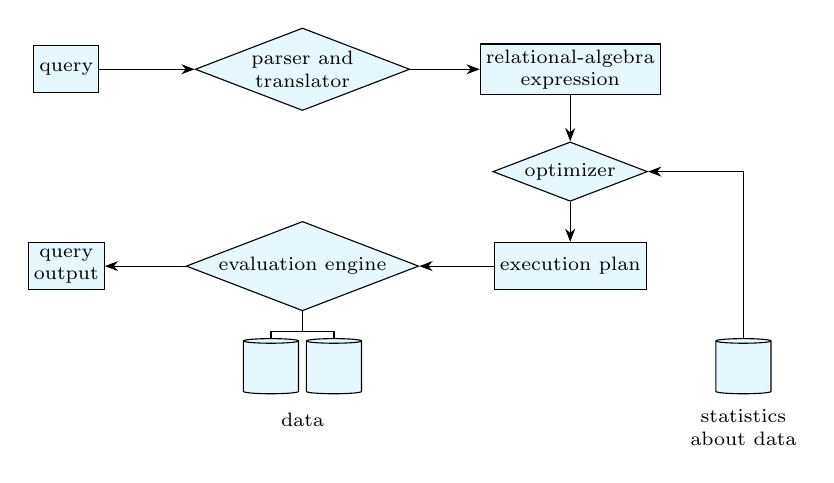
\begin{tikzpicture}[>=Stealth, font=\scriptsize,
  box/.style={draw, fill=cyan!10, align=center, minimum height=6mm, inner sep=2pt},
  dia/.style={draw, diamond, aspect=2.6, fill=cyan!10, align=center, inner sep=1pt},
  db/.style={draw, cylinder, shape border rotate=90, aspect=0.25, fill=cyan!10, minimum width=7mm, minimum height=7mm}]
\node[box] (q) at (0,0) {query};
\node[dia] (p) at (3,0) {parser and\\translator};
\node[box] (ra) at (6.4,0) {relational-algebra\\expression};
\node[dia] (o) at (6.4,-1.3) {optimizer};
\node[box] (ep) at (6.4,-2.5) {execution plan};
\node[dia] (ev) at (3,-2.5) {evaluation engine};
\node[box] (out) at (0,-2.5) {query\\output};
\node[db] (d1) at (2.6,-3.8) {}; \node[db] (d2) at (3.4,-3.8) {};
\node at (3,-4.45) {data};
\node[db] (st) at (8.6,-3.8) {}; \node[align=center] at (8.6,-4.55) {statistics\\about data};
\draw[->] (q) -- (p); \draw[->] (p) -- (ra); \draw[->] (ra) -- (o); \draw[->] (o) -- (ep);
\draw[->] (ep) -- (ev); \draw[->] (ev) -- (out);
\draw (ev.south) -- ++(0,-0.25) -| (d1.north); \draw (ev.south) -- ++(0,-0.25) -| (d2.north);
\draw[->] (st.north) |- (o.east);
\end{tikzpicture}
\end{center}

\begin{tabularx}{\linewidth}{@{}l X@{}}
\toprule
\textbf{Step} & \textbf{What happens}\\\midrule
1. Parsing and translation & The \textbf{scanner} finds tokens (keywords, names), the \textbf{parser} checks syntax, and the query is \textbf{validated} (do the relations and attributes exist?). It is then translated into an internal form: a relational algebra expression, i.e.\ a query tree or graph.\\
2. Optimization & The optimizer rewrites the expression and chooses algorithms and access paths (indexes, sort order). It uses \textbf{statistics about the data} (number of tuples, distinct values, index availability) to produce an \textbf{execution plan}.\\
3. Evaluation & The \textbf{evaluation engine} (runtime database processor) runs the plan against the data and returns the query output.\\
\bottomrule
\end{tabularx}

\subsection{Process for heuristic optimization (slide 268)}
\begin{enumerate}
  \item The \textbf{parser} of a high-level query generates an \textbf{initial internal representation} (the canonical query tree).
  \item \textbf{Heuristic rules} are applied to optimize this internal representation.
  \item A \textbf{query execution plan} is generated to execute groups of operations, based on the \textbf{access paths} available on the files involved in the query.
\end{enumerate}

\begin{keybox}[The main heuristic]
Apply first the operations that \textbf{reduce the size of intermediate results}. For example, apply \textbf{SELECT} ($\sigma$) and \textbf{PROJECT} ($\pi$) \textbf{before} the \textbf{JOIN} or other binary operations.
\end{keybox}

\textbf{Why it works:} a binary operation such as $\times$ or $\bowtie$ is expensive in proportion to the \emph{sizes} of its inputs. $\sigma$ shrinks the number of \textbf{rows}, and $\pi$ shrinks the \textbf{width} of each row (so more rows fit per block). Doing them early means every later operation handles far less data.

\begin{tabularx}{\linewidth}{@{}X X@{}}
\toprule
\textbf{Heuristic (rule-based) optimization} & \textbf{Cost-based optimization}\\\midrule
Applies \textbf{transformation rules} that usually improve the query tree, without estimating costs. & Estimates the \textbf{cost} of alternative plans from catalog statistics and picks the cheapest.\\
Fast; good for simple queries; always improves the canonical tree. & More accurate but more work; used by real DBMSs, usually \emph{after} heuristic rewriting.\\
\bottomrule
\end{tabularx}
\smallskip
(The slides cover heuristic optimization; cost-based optimization is shown here for contrast only.)

%=====================================================================
\section{Query Representation: Query Tree and Query Graph}

\begin{tabularx}{\linewidth}{@{}p{0.47\linewidth} X@{}}
\toprule
\textbf{Query tree} & \textbf{Query graph}\\\midrule
A tree data structure that corresponds to a \textbf{relational algebra} expression. & A graph data structure that corresponds to a \textbf{relational calculus} expression.\\
\textbf{Leaf nodes} = input relations; \textbf{internal nodes} = RA operations. & \textbf{Relation nodes} (single circles) and \textbf{constant nodes} (double circles); \textbf{edges} = selection and join conditions; attributes to retrieve shown in [ ].\\
Execution: run an internal node as soon as its operands are available, and \textbf{replace that node} by the resulting relation. Execution ends when the \textbf{root} is executed. & Does \textbf{not} indicate an order in which to perform operations.\\
\textbf{Many} trees for one query (fixes an order of evaluation). & Only a \textbf{single} graph for each query.\\
Preferred by optimizers, because the order is explicit. & Less used, because it cannot express an execution order.\\
\bottomrule
\end{tabularx}

\subsection{Translation first: query blocks (slide 270)}
Before optimizing, the SQL query is translated into RA (see the separate \emph{SQL to Relational Algebra} notes).
\begin{itemize}
  \item A \textbf{query block} is the basic unit that is translated into algebraic operators and optimized. It contains a single \texttt{SELECT-FROM-WHERE} expression, plus \texttt{GROUP BY} and \texttt{HAVING} if they are part of the block.
  \item \textbf{Nested queries} are identified as \textbf{separate query blocks}. Aggregate operators must be included in the \textbf{extended algebra}.
  \item Example (slide 271): \texttt{SELECT LNAME, FNAME FROM EMPLOYEE WHERE SALARY > (SELECT MAX(SALARY) FROM EMPLOYEE WHERE DNO = 5)} splits into the inner block $\mathcal{F}_{MAX\ SALARY}(\sigma_{DNO=5}(\R{EMPLOYEE}))$, giving a constant $c$, and the outer block $\pi_{LNAME,FNAME}(\sigma_{SALARY>c}(\R{EMPLOYEE}))$. Each block is optimized separately.
\end{itemize}

\subsection{Example Q2: query tree and query graph (slides 272--274)}
\begin{exbox}[Q2]
\emph{For every project located in `Stafford', retrieve the project number, the controlling department number, and the department manager's last name, address and birth date.}
\begin{verbatim}
SELECT P.PNUMBER, P.DNUM, E.LNAME, E.ADDRESS, E.BDATE
FROM   PROJECT AS P, DEPARTMENT AS D, EMPLOYEE AS E
WHERE  P.DNUM = D.DNUMBER AND D.MGRSSN = E.SSN AND P.PLOCATION = 'Stafford';
\end{verbatim}
\begin{multline*}
\pi_{PNUMBER,DNUM,LNAME,ADDRESS,BDATE}\Big(\big(\big(\sigma_{PLOCATION=\text{'Stafford'}}(\R{PROJECT})\big)\\
\bowtie_{DNUM=DNUMBER} \R{DEPARTMENT}\big) \bowtie_{MGRSSN=SSN} \R{EMPLOYEE}\Big)
\end{multline*}
\end{exbox}

\begin{center}
\begin{minipage}[t]{0.5\linewidth}\centering
{\footnotesize\bfseries (a) Query tree for the RA expression}\\[2pt]
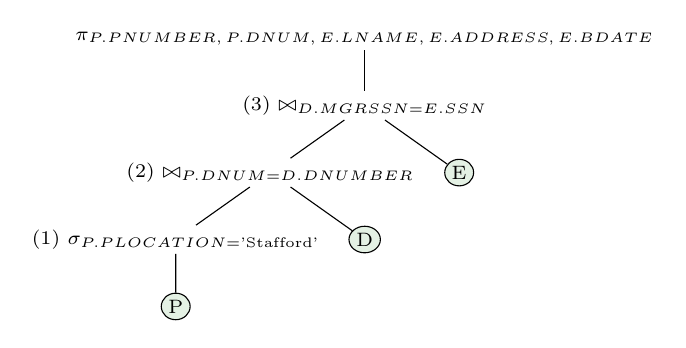
\begin{tikzpicture}[qt, level 1/.style={sibling distance=28mm}, level 2/.style={sibling distance=24mm}]
\node {$\pi_{P.PNUMBER,\,P.DNUM,\,E.LNAME,\,E.ADDRESS,\,E.BDATE}$}
  child {node {(3)\ $\bowtie_{D.MGRSSN=E.SSN}$}
    child {node {(2)\ $\bowtie_{P.DNUM=D.DNUMBER}$}
      child {node {(1)\ $\sigma_{P.PLOCATION=\text{'Stafford'}}$}
        child {node[rel] {P}}}
      child {node[rel] {D}}}
    child {node[rel] {E}}};
\end{tikzpicture}
\end{minipage}\hfill
\begin{minipage}[t]{0.48\linewidth}\centering
{\footnotesize\bfseries (b) Initial (canonical) query tree for the SQL}\\[2pt]
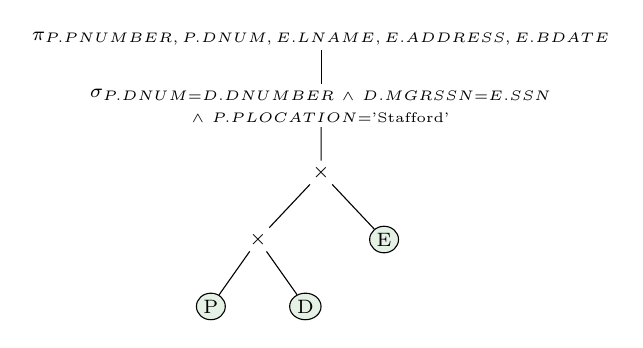
\begin{tikzpicture}[qt, level 3/.style={sibling distance=16mm}, level 4/.style={sibling distance=12mm}]
\node {$\pi_{P.PNUMBER,\,P.DNUM,\,E.LNAME,\,E.ADDRESS,\,E.BDATE}$}
  child {node[align=center] {$\sigma_{P.DNUM=D.DNUMBER\ \wedge\ D.MGRSSN=E.SSN}$\\$_{\wedge\ P.PLOCATION=\text{'Stafford'}}$}
    child {node {$\times$}
      child {node {$\times$}
        child {node[rel] {P}}
        child {node[rel] {D}}}
      child {node[rel] {E}}}};
\end{tikzpicture}
\end{minipage}

\medskip
{\footnotesize\bfseries (c) Query graph for Q2}\\[2pt]
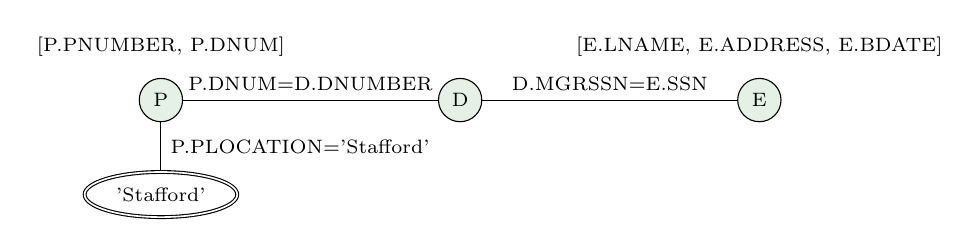
\begin{tikzpicture}[font=\scriptsize]
\node[rel, circle, minimum size=5.5mm] (P) at (0,0) {P};
\node[rel, circle, minimum size=5.5mm] (D) at (3.8,0) {D};
\node[rel, circle, minimum size=5.5mm] (E) at (7.6,0) {E};
\node[draw, double, ellipse] (S) at (0,-1.2) {'Stafford'};
\draw (P) -- node[above] {P.DNUM=D.DNUMBER} (D);
\draw (D) -- node[above] {D.MGRSSN=E.SSN} (E);
\draw (P) -- node[right] {P.PLOCATION='Stafford'} (S);
\node[above=1.5mm of P] {[P.PNUMBER, P.DNUM]};
\node[above=1.5mm of E] {[E.LNAME, E.ADDRESS, E.BDATE]};
\end{tikzpicture}
\end{center}

\begin{itemize}
  \item Tree (a) executes bottom-up in the numbered order: (1) select the Stafford projects, (2) join with DEPARTMENT, (3) join with EMPLOYEE, then project.
  \item Tree (b) is what the parser produces directly: $\times$ of all FROM tables, one big $\sigma$, one $\pi$. It is \textbf{correct but very inefficient}. Heuristic optimization turns (b) into something like (a).
\end{itemize}

%=====================================================================
\section{Heuristic Optimization of Query Trees}

\begin{keybox}[Idea (slide 275)]
\begin{itemize}
  \item The same query can correspond to \textbf{many different relational algebra expressions}, and hence \textbf{many different query trees}, all giving the same answer.
  \item The task of heuristic optimization is to transform the initial tree into a \textbf{final query tree that is efficient to execute}, using transformation rules that are guaranteed to preserve the result (Section~\ref{sec:rules}).
\end{itemize}
\end{keybox}

\subsection{Steps in optimizing a query tree (slide 276)}
\begin{enumerate}
  \item \textbf{Move SELECT operations down} the query tree (as close to the leaves as possible).
  \item \textbf{Apply the more restrictive SELECT operation first} (reorder the leaves so that the relations with the smallest selections are processed first).
  \item \textbf{Replace CARTESIAN PRODUCT and SELECT with JOIN} operations.
  \item \textbf{Move PROJECT operations down} the tree (keep only the attributes needed higher up).
\end{enumerate}

\subsection{Worked example (slides 276--279, Fig.~18.5)}
\begin{exbox}[Query Q]
\emph{Find the last names of employees born after 1957 who work on a project named `Aquarius'.}
\begin{verbatim}
SELECT LNAME
FROM   EMPLOYEE, WORKS_ON, PROJECT
WHERE  PNAME = 'Aquarius' AND PNUMBER = PNO AND ESSN = SSN AND BDATE > '1957-12-31';
\end{verbatim}
Conditions: $PNAME=\aq$ and $BDATE>\bd$ are \textbf{selections} (one table each). $PNUMBER=PNO$ (PROJECT--WORKS\_ON) and $ESSN=SSN$ (WORKS\_ON--EMPLOYEE) are \textbf{join conditions}.
\end{exbox}

\subsubsection*{(a) Initial (canonical) query tree}
\begin{minipage}[c]{0.46\linewidth}\centering
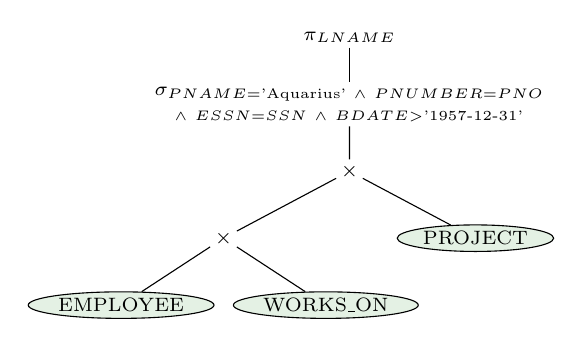
\begin{tikzpicture}[qt, level 3/.style={sibling distance=32mm}, level 4/.style={sibling distance=26mm}]
\node {$\pi_{LNAME}$}
  child {node[align=center] {$\sigma_{PNAME=\aq\ \wedge\ PNUMBER=PNO}$\\$_{\wedge\ ESSN=SSN\ \wedge\ BDATE>\bd}$}
    child {node {$\times$}
      child {node {$\times$}
        child {node[rel] {EMPLOYEE}}
        child {node[rel] {WORKS\_ON}}}
      child {node[rel] {PROJECT}}}};
\end{tikzpicture}
\end{minipage}\hfill
\begin{minipage}[c]{0.5\linewidth}
\[ \pi_{LNAME}\big(\sigma_{C}((E \times W) \times P)\big) \]
($E$ = EMPLOYEE, $W$ = WORKS\_ON, $P$ = PROJECT, $C$ = the whole WHERE clause.)
The FROM tables are combined with $\times$ in the order written, then one $\sigma$ with the whole WHERE clause, then $\pi$.

\textbf{Cost:} with the textbook COMPANY data (8 employees, 16 WORKS\_ON rows, 6 projects), the product alone produces $8 \times 16 \times 6 = 768$ tuples, and each is as wide as all three relations together. In a real database with thousands of rows per table this is millions or billions of tuples.
\end{minipage}

\subsubsection*{(b) Step 1: move SELECT operations down}
\begin{minipage}[c]{0.5\linewidth}\centering
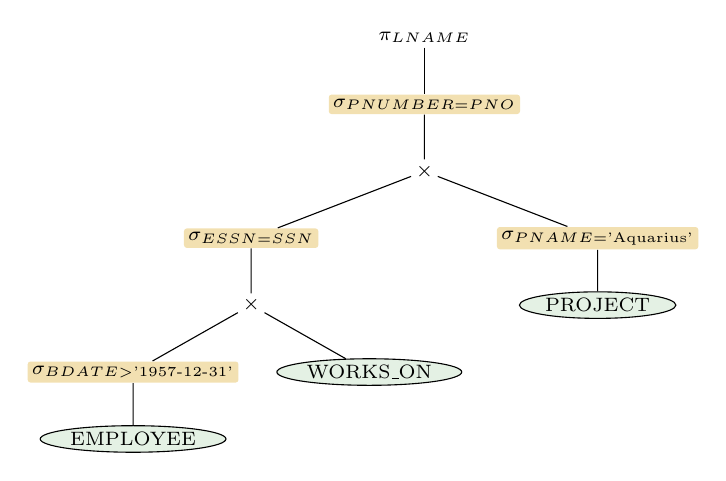
\begin{tikzpicture}[qt, level 3/.style={sibling distance=44mm}, level 5/.style={sibling distance=30mm}]
\node {$\pi_{LNAME}$}
  child {node[hot] {$\sigma_{PNUMBER=PNO}$}
    child {node {$\times$}
      child {node[hot] {$\sigma_{ESSN=SSN}$}
        child {node {$\times$}
          child {node[hot] {$\sigma_{BDATE>\bd}$}
            child {node[rel] {EMPLOYEE}}}
          child {node[rel] {WORKS\_ON}}}}
      child {node[hot] {$\sigma_{PNAME=\aq}$}
        child {node[rel] {PROJECT}}}}};
\end{tikzpicture}
\end{minipage}\hfill
\begin{minipage}[c]{0.46\linewidth}
\begin{itemize}
  \item Split the conjunctive $\sigma$ into four separate selections (\textbf{cascade of $\sigma$}, rule 1).
  \item Push each one down as far as its attributes allow (rules 2, 7).
  \item $\sigma_{BDATE}$ only uses EMPLOYEE, so it goes directly above EMPLOYEE. $\sigma_{PNAME}$ goes directly above PROJECT.
  \item $\sigma_{ESSN=SSN}$ needs EMPLOYEE and WORKS\_ON, so it sits just above their $\times$. $\sigma_{PNUMBER=PNO}$ needs WORKS\_ON and PROJECT, so it stays above the top $\times$.
\end{itemize}
\end{minipage}

\subsubsection*{(c) Step 2: apply the more restrictive SELECT first}
\begin{minipage}[c]{0.5\linewidth}\centering
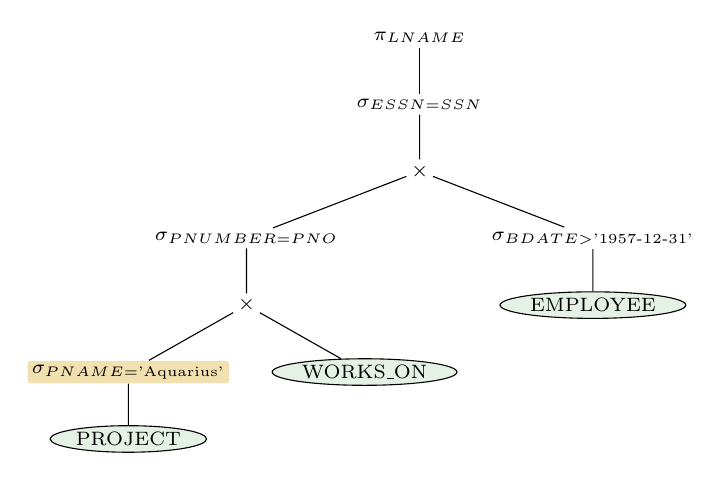
\begin{tikzpicture}[qt, level 3/.style={sibling distance=44mm}, level 5/.style={sibling distance=30mm}]
\node {$\pi_{LNAME}$}
  child {node {$\sigma_{ESSN=SSN}$}
    child {node {$\times$}
      child {node {$\sigma_{PNUMBER=PNO}$}
        child {node {$\times$}
          child {node[hot] {$\sigma_{PNAME=\aq}$}
            child {node[rel] {PROJECT}}}
          child {node[rel] {WORKS\_ON}}}}
      child {node {$\sigma_{BDATE>\bd}$}
        child {node[rel] {EMPLOYEE}}}}};
\end{tikzpicture}
\end{minipage}\hfill
\begin{minipage}[c]{0.46\linewidth}
\begin{itemize}
  \item $\sigma_{PNAME=\aq}$ is the \textbf{most restrictive}: PNAME is (nearly) unique, so it returns about \textbf{one} project. $\sigma_{BDATE>\bd}$ may return many employees.
  \item So the leaves are \textbf{rearranged}: PROJECT is processed first and combined with WORKS\_ON, and EMPLOYEE comes last. Rules 5, 6 and 10 (commutativity and associativity) allow the reordering.
  \item The rearrangement also avoids a \textbf{pure} Cartesian product: every $\times$ now has a join condition directly above it.
\end{itemize}
\end{minipage}

\subsubsection*{(d) Step 3: replace CARTESIAN PRODUCT and SELECT with JOIN}
\begin{minipage}[c]{0.5\linewidth}\centering
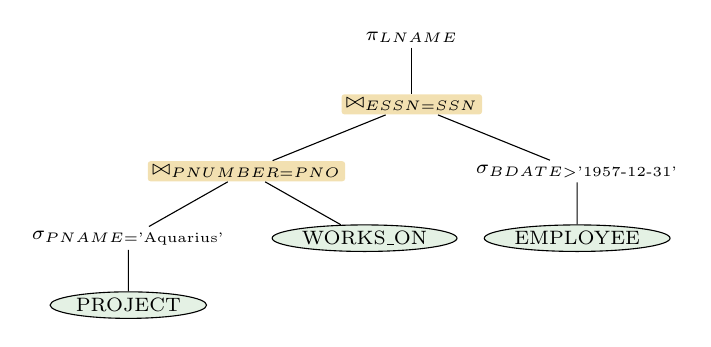
\begin{tikzpicture}[qt, level 2/.style={sibling distance=42mm}, level 3/.style={sibling distance=30mm}]
\node {$\pi_{LNAME}$}
  child {node[hot] {$\bowtie_{ESSN=SSN}$}
    child {node[hot] {$\bowtie_{PNUMBER=PNO}$}
      child {node {$\sigma_{PNAME=\aq}$}
        child {node[rel] {PROJECT}}}
      child {node[rel] {WORKS\_ON}}}
    child {node {$\sigma_{BDATE>\bd}$}
      child {node[rel] {EMPLOYEE}}}};
\end{tikzpicture}
\end{minipage}\hfill
\begin{minipage}[c]{0.46\linewidth}
\begin{itemize}
  \item Every $\sigma_{\theta}$ that sits directly above a $\times$ with a join condition $\theta$ becomes a join: $\sigma_\theta(E_1 \times E_2) = E_1 \bowtie_\theta E_2$ (rule 4).
  \item Joins can use efficient algorithms (index lookups, sort-merge, hash join) and never build the full product.
\end{itemize}
\end{minipage}

\subsubsection*{(e) Step 4: move PROJECT operations down}
\begin{minipage}[c]{0.56\linewidth}\centering
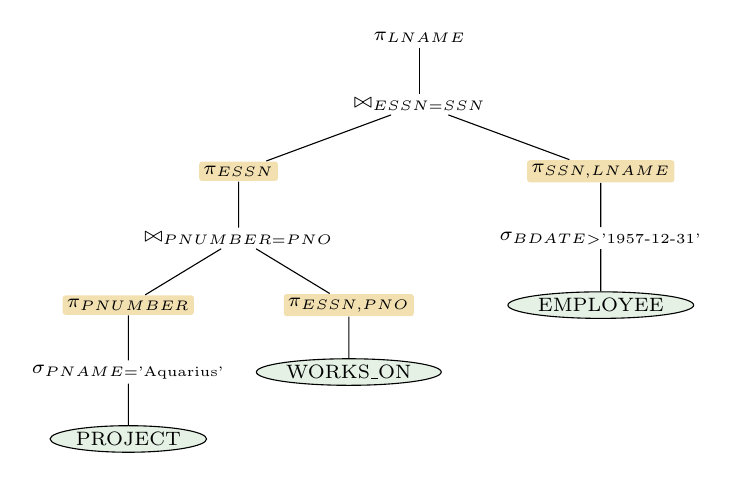
\begin{tikzpicture}[qt, level 2/.style={sibling distance=46mm}, level 4/.style={sibling distance=28mm}]
\node {$\pi_{LNAME}$}
  child {node {$\bowtie_{ESSN=SSN}$}
    child {node[hot] {$\pi_{ESSN}$}
      child {node {$\bowtie_{PNUMBER=PNO}$}
        child {node[hot] {$\pi_{PNUMBER}$}
          child {node {$\sigma_{PNAME=\aq}$}
            child {node[rel] {PROJECT}}}}
        child {node[hot] {$\pi_{ESSN,PNO}$}
          child {node[rel] {WORKS\_ON}}}}}
    child {node[hot] {$\pi_{SSN,LNAME}$}
      child {node {$\sigma_{BDATE>\bd}$}
        child {node[rel] {EMPLOYEE}}}}};
\end{tikzpicture}
\end{minipage}\hfill
\begin{minipage}[c]{0.4\linewidth}
\begin{itemize}
  \item Above each node keep only the attributes needed \textbf{later}: in join conditions or the final result (rules 3, 8).
  \item From PROJECT only \texttt{PNUMBER} is needed (for $PNUMBER=PNO$). From WORKS\_ON only \texttt{ESSN, PNO}. After that join, only \texttt{ESSN}. From EMPLOYEE only \texttt{SSN} (join) and \texttt{LNAME} (result).
  \item Intermediate tuples become much \textbf{narrower}.
\end{itemize}
\end{minipage}

\medskip
\begin{exbox}[Final optimized expression]
\begin{multline*}
\pi_{LNAME}\bigg(\pi_{ESSN}\Big(\pi_{PNUMBER}\big(\sigma_{PNAME=\aq}(\R{PROJECT})\big)\\
\bowtie_{PNUMBER=PNO} \pi_{ESSN,PNO}(\R{WORKS\_ON})\Big)\\
\bowtie_{ESSN=SSN}\ \pi_{SSN,LNAME}\big(\sigma_{BDATE>\bd}(\R{EMPLOYEE})\big)\bigg)
\end{multline*}
Compare with the canonical $\pi_{LNAME}(\sigma_C(\R{EMPLOYEE} \times \R{WORKS\_ON} \times \R{PROJECT}))$: same result, far less work.
\end{exbox}

%=====================================================================
\section{Transformation Rules for Relational Algebra}\label{sec:rules}

Two RA expressions are \textbf{equivalent} if they produce the same set of tuples on \emph{every} legal database instance. These rules (slides 280--283) are what make each optimization step legal. $E$, $E_1$, $E_2$, $E_3$ are RA expressions, $\theta$ are conditions and $L$ are attribute lists.

\begin{keybox}[Rules on selection and projection]
\textbf{1. Cascade of $\sigma$.} A conjunctive selection can be broken into a sequence of individual selections:
\[ \sigma_{\theta_1 \wedge \theta_2}(E) = \sigma_{\theta_1}(\sigma_{\theta_2}(E)) \]
\textbf{2. Commutativity of $\sigma$.}
\[ \sigma_{\theta_1}(\sigma_{\theta_2}(E)) = \sigma_{\theta_2}(\sigma_{\theta_1}(E)) \]
\textbf{3. Cascade of $\pi$.} Only the final projection in a sequence is needed; the others can be omitted:
\[ \pi_{L_1}(\pi_{L_2}(\dots(\pi_{L_n}(E))\dots)) = \pi_{L_1}(E) \qquad (L_1 \subseteq L_2 \subseteq \dots \subseteq L_n) \]
\textbf{Used for:} rule 1 splits the big WHERE $\sigma$ into pieces, and rule 2 lets each piece slide past the others on its way down.
\end{keybox}

\begin{keybox}[Rules on joins and products]
\textbf{4. Selections combine with Cartesian products and theta joins.}
\[ \sigma_{\theta}(E_1 \times E_2) = E_1 \bowtie_{\theta} E_2 \qquad\qquad \sigma_{\theta_1}(E_1 \bowtie_{\theta_2} E_2) = E_1 \bowtie_{\theta_1 \wedge \theta_2} E_2 \]
\textbf{5. Theta join (and $\times$) is commutative.}
\[ E_1 \bowtie_{\theta} E_2 = E_2 \bowtie_{\theta} E_1 \]
\textbf{6. Natural join is associative.}
\[ (E_1 \bowtie E_2) \bowtie E_3 = E_1 \bowtie (E_2 \bowtie E_3) \]
Theta joins are associative in the following manner, where $\theta_2$ involves attributes from $E_2$ and $E_3$ only:
\[ (E_1 \bowtie_{\theta_1} E_2) \bowtie_{\theta_2 \wedge \theta_3} E_3 = E_1 \bowtie_{\theta_1 \wedge \theta_3} (E_2 \bowtie_{\theta_2} E_3) \]
\textbf{Used for:} rule 4 is step 3 (product + selection $\to$ join). Rules 5 and 6 allow the join order to be rearranged (step 2).
\end{keybox}

\begin{keybox}[Distribution over joins]
\textbf{7. $\sigma$ distributes over the theta join} under two conditions:

(a) when all attributes in $\theta_0$ involve only the attributes of \textbf{one} of the expressions ($E_1$) being joined:
\[ \sigma_{\theta_0}(E_1 \bowtie_{\theta} E_2) = (\sigma_{\theta_0}(E_1)) \bowtie_{\theta} E_2 \]
(b) when $\theta_1$ involves only attributes of $E_1$ and $\theta_2$ only attributes of $E_2$:
\[ \sigma_{\theta_1 \wedge \theta_2}(E_1 \bowtie_{\theta} E_2) = (\sigma_{\theta_1}(E_1)) \bowtie_{\theta} (\sigma_{\theta_2}(E_2)) \]
\textbf{8. $\pi$ distributes over the theta join.} Let $L_1$ and $L_2$ be attributes of $E_1$ and $E_2$.

(a) If the join condition $\theta$ involves only attributes in $L_1 \cup L_2$:
\[ \pi_{L_1 \cup L_2}(E_1 \bowtie_{\theta} E_2) = (\pi_{L_1}(E_1)) \bowtie_{\theta} (\pi_{L_2}(E_2)) \]
(b) In general, let $L_3$ be the attributes of $E_1$ used in $\theta$ but not in $L_1 \cup L_2$, and $L_4$ the attributes of $E_2$ used in $\theta$ but not in $L_1 \cup L_2$. Then:
\[ \pi_{L_1 \cup L_2}(E_1 \bowtie_{\theta} E_2) = \pi_{L_1 \cup L_2}\big((\pi_{L_1 \cup L_3}(E_1)) \bowtie_{\theta} (\pi_{L_2 \cup L_4}(E_2))\big) \]
\textbf{Used for:} rule 7 pushes $\sigma$ down (step 1). Rule 8 pushes $\pi$ down (step 4). In 8(b) the join attributes $L_3, L_4$ must be kept below the join and dropped only above it, which is why tree (e) keeps \texttt{PNUMBER}, \texttt{PNO} and \texttt{SSN} until their joins are done.
\end{keybox}

\begin{keybox}[Rules on set operations]
\textbf{9. Union and intersection are commutative} (set difference is \textbf{not}):
\[ E_1 \cup E_2 = E_2 \cup E_1 \qquad\qquad E_1 \cap E_2 = E_2 \cap E_1 \]
\textbf{10. Union and intersection are associative.}
\[ (E_1 \cup E_2) \cup E_3 = E_1 \cup (E_2 \cup E_3) \qquad\qquad (E_1 \cap E_2) \cap E_3 = E_1 \cap (E_2 \cap E_3) \]
\textbf{11. $\sigma$ distributes over $\cup$, $\cap$ and $-$.} For $\ominus \in \{\cup, \cap, -\}$: $\sigma_P(E_1 \ominus E_2) = \sigma_P(E_1) \ominus \sigma_P(E_2)$. For $\cap$ and $-$ it is enough to select on $E_1$ only:
\[ \sigma_P(E_1 - E_2) = \sigma_P(E_1) - E_2 = \sigma_P(E_1) - \sigma_P(E_2) \]
(This does \textbf{not} hold for $\cup$: $\sigma_P(E_1 \cup E_2) \neq \sigma_P(E_1) \cup E_2$.)

\textbf{12. $\pi$ distributes over $\cup$.}
\[ \pi_L(E_1 \cup E_2) = (\pi_L(E_1)) \cup (\pi_L(E_2)) \]
($\pi$ does \textbf{not} distribute over $\cap$ or $-$ in general.)
\end{keybox}

\begin{exbox}[Why $\pi$ does not distribute over $-$]
$E_1 = \{(1,a)\}$, $E_2 = \{(1,b)\}$ with attributes $(A,B)$. Then $\pi_A(E_1 - E_2) = \pi_A(\{(1,a)\}) = \{1\}$, but $\pi_A(E_1) - \pi_A(E_2) = \{1\} - \{1\} = \emptyset$.
\end{exbox}

%=====================================================================
\section{The Heuristic Optimization Algorithm (Summary)}

Elmasri \& Navathe's outline, which is the four slide steps written as rule applications:
\begin{enumerate}
  \item \textbf{Break up} conjunctive selections into a cascade of $\sigma$ (rule 1). \emph{This gives freedom to move each piece separately.}
  \item \textbf{Move each $\sigma$ as far down} the tree as its attributes allow (rules 2, 4, 7, 11).
  \item \textbf{Rearrange the leaf nodes} so that the \textbf{most restrictive} selections are executed first, i.e.\ those producing the fewest tuples or the smallest relation. Avoid orders that lead to a pure Cartesian product (rules 5, 6, 9, 10).
  \item \textbf{Combine} a $\times$ with a $\sigma$ above it that holds a join condition into a \textbf{join} (rule 4).
  \item \textbf{Break up and move lists of projection attributes down} the tree as far as possible, creating new $\pi$ operations where needed (rules 3, 8, 12).
  \item \textbf{Identify subtrees} that are groups of operations executable by a single algorithm (for example a $\sigma$ + $\bowtie$ + $\pi$ pipeline) and generate the execution plan.
\end{enumerate}

\begin{keybox}[One-line summary]
\textbf{Selections down, restrictive first, products become joins, projections down.} Every step shrinks intermediate results, either fewer rows ($\sigma$, joins instead of $\times$) or narrower rows ($\pi$).
\end{keybox}

%=====================================================================
\section{Practice: Optimize a Query}

\begin{exbox}[Exercise]
\texttt{SELECT E.FNAME, E.LNAME FROM EMPLOYEE E, DEPARTMENT D WHERE D.DNAME = 'Research' AND D.DNUMBER = E.DNO AND E.SALARY > 30000;}

Draw the canonical tree and optimize it step by step.
\end{exbox}

\begin{center}
\begin{minipage}[t]{0.32\linewidth}\centering
{\footnotesize\bfseries Canonical}\\[2pt]
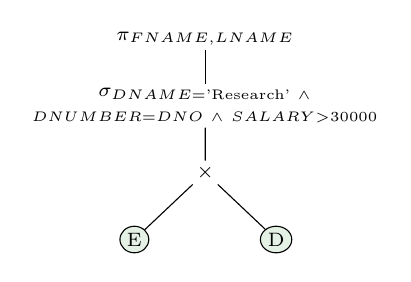
\begin{tikzpicture}[qt, level 3/.style={sibling distance=18mm}]
\node {$\pi_{FNAME,LNAME}$}
  child {node[align=center] {$\sigma_{DNAME=\text{'Research'}\ \wedge}$\\$_{DNUMBER=DNO\ \wedge\ SALARY>30000}$}
    child {node {$\times$}
      child {node[rel] {E}}
      child {node[rel] {D}}}};
\end{tikzpicture}
\end{minipage}\hfill
\begin{minipage}[t]{0.32\linewidth}\centering
{\footnotesize\bfseries Steps 1--3: $\sigma$ down, join}\\[2pt]
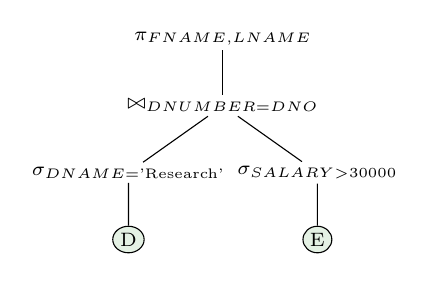
\begin{tikzpicture}[qt, level 2/.style={sibling distance=24mm}]
\node {$\pi_{FNAME,LNAME}$}
  child {node {$\bowtie_{DNUMBER=DNO}$}
    child {node {$\sigma_{DNAME=\text{'Research'}}$}
      child {node[rel] {D}}}
    child {node {$\sigma_{SALARY>30000}$}
      child {node[rel] {E}}}};
\end{tikzpicture}
\end{minipage}\hfill
\begin{minipage}[t]{0.32\linewidth}\centering
{\footnotesize\bfseries Step 4: $\pi$ down}\\[2pt]
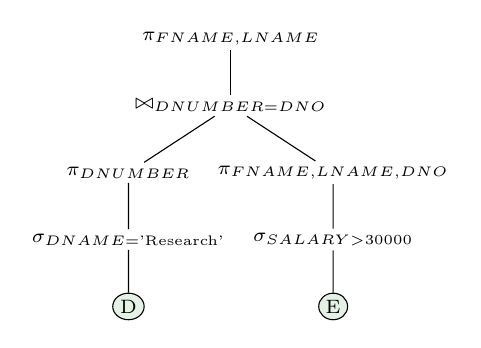
\begin{tikzpicture}[qt, level 2/.style={sibling distance=26mm}]
\node {$\pi_{FNAME,LNAME}$}
  child {node {$\bowtie_{DNUMBER=DNO}$}
    child {node {$\pi_{DNUMBER}$}
      child {node {$\sigma_{DNAME=\text{'Research'}}$}
        child {node[rel] {D}}}}
    child {node {$\pi_{FNAME,LNAME,DNO}$}
      child {node {$\sigma_{SALARY>30000}$}
        child {node[rel] {E}}}}};
\end{tikzpicture}
\end{minipage}
\end{center}

\begin{itemize}
  \item $\sigma_{DNAME='Research'}$ gives \textbf{one} department, so D is placed first (the most restrictive selection).
  \item With the COMPANY data (8 employees, 3 departments), the canonical product has $8 \times 3 = 24$ tuples. After optimization the join combines \textbf{1} department tuple with the \textbf{4} employees earning over 30000 (Wong, Wallace, Narayan, Borg), and \textbf{2} tuples come out: Franklin Wong and Ramesh Narayan. Smith earns exactly 30000, so he fails $SALARY > 30000$.
  \item Final:
\begin{multline*}
\pi_{FNAME,LNAME}\Big(\pi_{DNUMBER}\big(\sigma_{DNAME=\text{'Research'}}(\R{DEPARTMENT})\big)\\
\bowtie_{DNUMBER=DNO} \pi_{FNAME,LNAME,DNO}\big(\sigma_{SALARY>30000}(\R{EMPLOYEE})\big)\Big)
\end{multline*}
\end{itemize}

%=====================================================================
\section{Errors in the Slides}

\begin{warnbox}[Corrections]
\small
\begin{tabularx}{\linewidth}{@{}l X@{}}
\toprule
\textbf{Slide} & \textbf{Issue $\to$ correct version}\\\midrule
276 & ``PNMUBER'' $\to$ \textbf{PNUMBER}. The SQL writes `AQUARIUS' and `1957-12-31', while the trees (Fig.~18.5) write `Aquarius' and `DEC-31-1957'. They mean the same values.\\
281 & Rule 4: ``$\sigma_{\theta_1}(E_1 \bowtie_{\sigma_{\theta_2}} E_2)$'' has a stray $\sigma$ in the join subscript $\to$ $\sigma_{\theta_1}(E_1 \bowtie_{\theta_2} E_2) = E_1 \bowtie_{\theta_1 \wedge \theta_2} E_2$.\\
283 & Rule 11 shows only the $-$ case. $\sigma$ also distributes over $\cup$ and $\cap$, but the shortcut $\sigma_P(E_1) \ominus E_2$ is valid only for $-$ and $\cap$, not for $\cup$.\\
272 & ``P.NUMBER'' $\to$ P.\textbf{PNUMBER}; ``‘ STAFFORD ’'' has stray spaces.\\
\bottomrule
\end{tabularx}
\end{warnbox}

%=====================================================================
\section{Quick Revision}

\begin{itemize}
  \item \textbf{Query optimization} = choosing a suitable execution strategy. Internal forms: \textbf{query tree} (RA, leaves = relations, internal nodes = operators, many per query) and \textbf{query graph} (relational calculus, no order, one per query).
  \item \textbf{Query processing:} parsing and translation $\to$ optimization (uses statistics) $\to$ evaluation. \textbf{Query block} = one SELECT-FROM-WHERE (+ GROUP BY/HAVING), and nested queries are separate blocks.
  \item \textbf{Heuristic process:} parser builds the initial tree $\to$ heuristic rules improve it $\to$ execution plan based on access paths.
  \item \textbf{Main heuristic:} apply $\sigma$ and $\pi$ \textbf{before} joins and other binary operations, to reduce intermediate results.
  \item \textbf{Four steps:} (1) move $\sigma$ down, (2) most restrictive $\sigma$ first, (3) $\times$ + $\sigma$ $\to$ $\bowtie$, (4) move $\pi$ down.
  \item \textbf{Key rules:} cascade/commute of $\sigma$ (1, 2); cascade of $\pi$ (3); $\sigma(\times) = \bowtie$ (4); $\bowtie$ commutative and associative (5, 6); $\sigma$ and $\pi$ distribute over $\bowtie$ (7, 8); $\cup$, $\cap$ commutative and associative, $-$ is not (9, 10); $\sigma$ distributes over $\cup, \cap, -$ (11); $\pi$ distributes over $\cup$ (12).
  \item \textbf{Aquarius example:} canonical $\pi(\sigma(E \times W \times P))$ $\to$ $\pi_{LNAME}(\pi_{ESSN}(\pi_{PNUMBER}(\sigma_{PNAME}(P)) \bowtie \pi_{ESSN,PNO}(W)) \bowtie \pi_{SSN,LNAME}(\sigma_{BDATE}(E)))$.
\end{itemize}

\end{document}
